%%%%%%%%% PROJECT DESCRIPTION  -- 15 pages (including Prior NSF Support)

\required{Project Description}
\begin{center}
%\emph{Maximum of 15 pages}
\end{center}
%The Project Description (including Results from Prior NSF Support, which is
%limited to five pages) may not exceed 15 pages. Visual materials, including charts,
%graphs, maps, photographs and other pictorial presentations are included in the
%15-page limitation. PIs be cautioned that the project description must
%be self-contained and that URLs that provide information related to the proposal
%should not be used. \\
%
%All proposals to NSF are reviewed utilizing the two merit review criteria,
%intellectual merit and broader impacts. \\
%
% The Project Description should provide a clear statement of the work 
% to be undertaken and must include: objectives for the period of the proposed 
% work and expected significance; relation to longer-term goals of the PI's 
% project; and relation to the present state of knowledge in the field, 
% to work in progress by the PI under other support and to work in progress 
% elsewhere.

%%%%%%%%%%%%%%%%%%%%%%%%%%%%%%%%%%%%%%%%%%%%%%%%%%%%%%%%%%%%%%%%%%%%%%
%INTRO
%%%%%%%%%%%%%%%%%%%%%%%%%%%%%%%%%%%%%%%%%%%%%%%%%%%%%%%%%%%%%%%%%%%%%%
\section*{Introduction}

Local adaptation occurs when natural selection prevails over gene flow and organisms achieve maximum fitness at their native sites \citep{Kawecki2004}. An understanding of local adaptation is particularly pressing given current issues of climate change, conservation, and sustainable agricultural production \citep{savolainen2013ecological}.   While the genetic basis of local adaptation is generally not well understood, the declining cost of next generation sequencing has enabled a handful of genome-wide studies across many populations of model species.  For example, \citet{fournier2011map} demonstrated that alleles associated with high fitness in \emph{Arabidopsis thaliana} had a tendency to be both local and linked to climate.  Likewise, a recent study across hundreds of accessions of \emph{Medicago truncatula} identified candidate loci for local adaptation and found them to be predictive for growth rate under temperature and soil moisture treatments in a growth chamber \citep{Yoder17012014}.  Finally, our genome-wide study of 21 populations of teosinte (wild relatives of maize) revealed that an important role for inversion polymorphisms and regulatory variants in adaptation across an elevational gradient \citep{Pyhajarvi2013}.  Clearly, initial genomic studies are yielding valuable insights regarding local adaptation, yet much remains to be discovered.

Agricultural species represent particularly promising systems for ongoing research on local adaptation.  Crops were, in most cases, domesticated in narrow geographic centers prior to global spread.  During diffusion, crops encountered and adapted to a wide range of novel environments and in many instances putative traits underlying such local adaptation have already been identified.  These systems therefore represent compelling opportunities for investigating the genetic architecture of local adaption.  Moreover, insights gained regarding adaptive loci can feed back into modern crop improvement yielding valuable benefits in the face of  rapid environmental change.

Here we propose an investigation of local adaptation in maize (\emph{Zea mays} ssp. \emph{mays}) to high elevation environments.  Maize was domesticated in the lowlands of southwest Mexico from the narrowly distributed teosinte \emph{Zea mays} ssp. \emph{parviglumis} \citep[hereafter, \emph{parviglumis}][]{Matsuoka2002}.  Following domestication, maize spread to the highlands of the Central Plateau, a migration across more than 1000m of increasing elevation to a dramatically different environment (CITE).  Maize landraces in the Central Plateau have distinct morphologies (e.g., highly pigmented and hairy leaves and stems) that are believed to confer adaptation to this cooler region (CITE).  Interestingly, these morphologies are also found in the highland-adapted teosinte \emph{Zea mays} ssp. \emph{mexicana} (hereafter, \emph{mexicana})(CITE).  Our recent work has shown that these shared traits are likely the result of adaptive introgression from \emph{mexicana} into maize \citep{Hufford2013}.  

Colonization of the Central Plateau is not the only occasion where highland adaptation was required during the diffusion of maize.  For example, landraces (i.e., local farmer varieties) of maize are commonly grown above 3000m in the Andes of South America.  Andean landraces share adaptive highland traits with landraces from the Central Plateau of Mexico, yet our previous genetic analysis clearly shows that colonization of the South American highlands occurred independently from local lowland landraces \citep{vanheerwaarden2011a}.  Moreover, Andean maize grows outside the distribution of \emph{mexicana} and all other teosinte and must therefore have obtained highland adaptation de novo or through standing variation.  The genetic basis of highland adaptation may therefore be quite distinct between the Central Plateau and the Andes.

% !NOTES: 
%perhaps throw in your teo paper in plos one somewhere? maybe below? mention that teo has the big advantage of having been there a long time and well adapted to environs.
%i think instead of e.g. pigmented, we cite the table \ref{tab:phenos} and fill it out.
%some CITES still missing
%should bring up teosinte as another parallel, as well as highland environs elsewhere.

%%%%%%%%%%%%%%%%%%%%%%%%%%%%%%%%%%%%%%%%%%%%%%%%%%%%%%%%%%%%%%%%%%%%%%
%AIMS
%%%%%%%%%%%%%%%%%%%%%%%%%%%%%%%%%%%%%%%%%%%%%%%%%%%%%%%%%%%%%%%%%%%%%%
\section*{Aims}

We will investigate the genetic basis of highland adaptation in maize by achieving three specific aims:

\begin{enumerate}
\item {\bf Genetic architecture of highland traits in maize}
\item {\bf Population genetic signatures of highland adaptation in maize and teosinte}
\item {\bf Functional characterization of adaptive quantitative trait loci}
\end{enumerate}

%%%%%%%%%%%%%%%%%%%%%%%%%%%%%%%%%%%%%%%%%%%%%%%%%%%%%%%%%%%%%%%%%%%%%%
%RAIONALE AND SIGNIFICANCE
%%%%%%%%%%%%%%%%%%%%%%%%%%%%%%%%%%%%%%%%%%%%%%%%%%%%%%%%%%%%%%%%%%%%%%
\section*{Rationale and Significance}
Maize is an exceptional model of post-domestication adaptation.  While \emph{parviglumis}, the progenitor of maize, is found only in the lowlands along the Pacific coast of southwest Mexico, maize is cultivated on six continents across wide latitudes, ranging from southern Chile to Canada (Tenaillon and Charcosset 2011).  In fact, our analysis of [describe data] indicates that maize is the most broadly cultivated crop globally (CITE Figure).  The spread of maize has required adaptation to a number of abiotic and biotic conditions including gradients of temperature, precipitation, and elevation.  Study of the genetic architecture of these adaptations will provide both basic evolutionary insight and essential information to help increase or sustain yield in the face of human population growth and climate change. Historical analyses suggest that climate change over the last 30 years has already dramatically impacted maize yields worldwide, slowing gains from breeding and management (Lobell et al. 2011a).  Based on data from historical maize trials and weather stations, Lobell and co-authors (2011b) determined that future temperature increases of 1 $^{\circ}$C would decrease yield across 65\% of African maize-growing regions.  One hundred percent of these regions will see diminished yield if increased temperature is accompanied by drought (Lobell et al. 2011b).  An understanding of how maize has adapted to challenging environmental conditions in the past will help mitigate yield loss due to future changes.


\begin{SCfigure}
  \centering
  \caption{Geographic breadth of the world's 16 most important crops. Geographic breadth is expressed in percent of land surface area in which each crop is cultiavated. Data from \citet{Ramankutty2008}. } 
   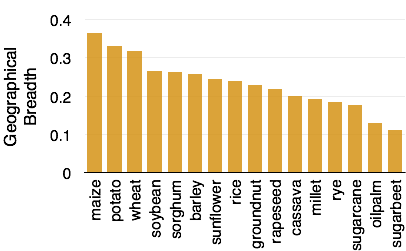
\includegraphics[width=0.5\textwidth]{breadth.png}
\label{fig:breadth}
\end{SCfigure}

\paragraph*{We know almost nothing about genetics adaptation in maize}


%MBH:  Don't think we need this point here, flows better after preliminary data
%we know lots about quant. traits in maize (temperate), but almost nothing about adaptive traits

%genetic arch. can differ. e.g. time to flowering in temp maize lots of genes small effect, but diff. between trop and temp is few photoperiod loci of large effect -- so adaptation to temperate was predominantly a few loci of large effect even though the genetic arch. of flowering time among temperate is lots of loci of small effect (reference fisher?) cite brown et al. 2011 \citep{Brown2011b} for differential architecture

%%%%%%%%%%%%%%%%%%%%%%%%%%%%%%%%%%%%%%%%%%%%%%%%%%%%%%%%%%%%%%%%%%%%%%
%PRELIMINARY RESULTS
%%%%%%%%%%%%%%%%%%%%%%%%%%%%%%%%%%%%%%%%%%%%%%%%%%%%%%%%%%%%%%%%%%%%%%
\section*{Preliminary Results}
% !HELP: writing

cite tanja for teosinte \citep{Pyhajarvi2013}
for maize, Huff 2013 \citep{Hufford2013}
shos stuff
van heerwaarden for independence \citep{Hufford2013}

describe current genome sequencing which will look at popgen and colonization

but none of this looks at quantitative traits (cite why quant. traits are different -- Rockman, lecorre \& kramer)

\begin{SCfigure}
  \centering \label{fig:fst}
   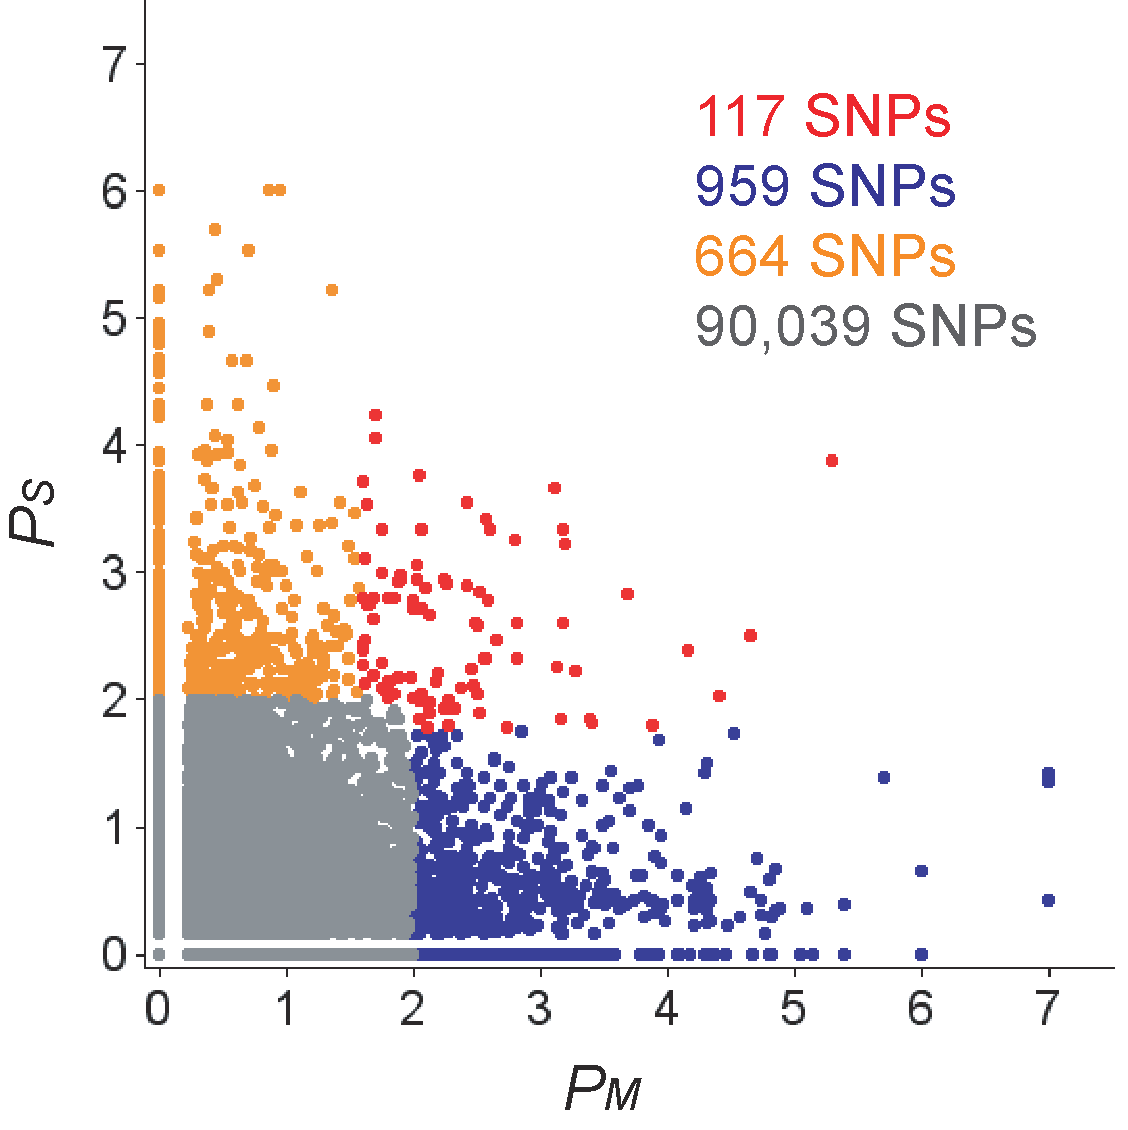
\includegraphics[width=0.4\textwidth]{fst.pdf}
  \caption{Scatter plot of $-\log_10 empirical P$-values of $F_{ST}$ values in Mexico ($P_M$ on $x$-axes) and South America ($P_S$ on $y$-axes).   Red, blue, orange and gray dots represents SNPs showing significance in both Mexico and South America, only in Mexico, or only in South America, respectively.  The number of SNPs in each category is shown in the same color of dots.} 
\end{SCfigure}


blah blah F$_ST$ \ref{fig:fst}.

%%%%%%%%%%%%%%%%%%%%%%%%%%%%%%%%%%%%%%%%%%%%%%%%%%%%%%%%%%%%%%%%%%%%%%
%SPECIFIC OBJECTIVES
%%%%%%%%%%%%%%%%%%%%%%%%%%%%%%%%%%%%%%%%%%%%%%%%%%%%%%%%%%%%%%%%%%%%%%
\section*{Specific Objectives}

%%%%%%%%%%%%%%%%%%%%%%%%%%%%%%%%%%%%%%%%%%%%%%%%%%%%%%%%%%%%%%%%%%%%%%
%AIM 1
%%%%%%%%%%%%%%%%%%%%%%%%%%%%%%%%%%%%%%%%%%%%%%%%%%%%%%%%%%%%%%%%%%%%%%

\renewcommand{\thesection}{Aim \arabic{section}}
\section{Genetic architecture of highland traits} \label{sec:qtl}

One of the primary goals of this proposal is to determine the genetic architecture of highland adaptation. Ultimately, this knowledge will be useful for determining the genes underlying these loci (\ref{sec:funchar}) and the pathways involved in adaptation (\ref{sec:selection}). These loci can also be used in maize improvement via marker assisted selection. In this aim we wish to determine how many genomic regions control adaptive phenotypes, where these regions are located, and the distribution of allelic effects at these loci. We first perform comparative QTL analysis in two highland x lowland crosses (\ref{subsec:qtlmap}), then take advantage of historical recombination and greater resolution to map loci in an admixed population of highland and lowland teosinte (\ref{subsec:admixmap}).

\subsection*{Questions}
\begin{itemize}[topsep=0pt,itemsep=-1ex,partopsep=1ex,parsep=1ex]
\item What is the genetic architecture of highland adaptation?
\item How much of the genetic architecture is shared between Mexico and South America?
\item How much of the genetic architecture is shared between maize and teosinte?
\item Are highland QTL/loci widespread in highland climes?
\end{itemize}

\subsection{QTL mapping of highland adaptation} \label{subsec:qtlmap}

The first objective of this project is to identify the genomic regions controlling highland adaptation in maize, we will conduct QTL mapping studies of one Mexican and one South American population, each derived by crossing an inbred landrace adapted to lowland conditions with a landrace adapted to highland conditions \ref{tab:qtlpops}.  We make use of specially-inbred landrace lines created by John Doebley (U. Wisconsin) and Seth Murray (Texas A\&M), thus simplifying downstream mapping applications and allowing replication of alleles in the our functional studies (see \ref{sec:funchar}). 

\begin{table}
\begin{center}
\caption{Parental lines for QTL} \label{tab:qtlpops}
\begin{tabular}{llll}\\\toprule  
{\bf Population}	& {\bf Parent } &	{\bf Origin (masl)} & {\bf Status }\\ \midrule
 \rowcolor{gray!25}
Mexico	& Zapalote Chico		& Oaxaca	 (46)		&  F2 \\ 
 \rowcolor{gray!25}
	& 	Palomero de Jalisco	& 	Jalisco (2520)		& \\
S. America	& Araguito	& Venezuela (183)	&  F1 \\ 
	& Sal Prieta	 & Ecuador (2948) & \\ \bottomrule
\end{tabular}
\end{center}
\end{table} 

Because we plan to evaluate these populations in replicated trials over multiple years, we will self-pollinate the F2 plants to create 500 F2:3 families from each population.  DNA will be extracted from each of the F2 plants and used for genotypic analysis.   The parents of the population will be sequenced to 20-30X depth on two lanes of Illumina (150bp paired-end reads on a HiSeq 2500 at the UC Davis Genome Center), providing genome-scale SNP data similar in scale (tens millions of markers) to our previous work in maize  \citep[HapMap.v2;][]{Chia2012a}.  F2 plants will be genotyped using genotyping-by-sequencing \citep[GBS;][]{Elshire2011} and run through the standard maize GBS pipeline \citep{Glaubitz2014} resulting in approximately \textasciitilde 1M SNPs and allowing simple imputation of full-genome sequence.  The genetic map will be created using standard methods \citep[e.g.][]{Broman2003a}. 

\begin{table}
\rowcolors{2}{gray!25}{white}
\begin{center}
\caption{Common garden locations} \label{tab:locales}
\begin{tabular}{p{2cm}cccccc}\\\toprule  
{\bf Field Sites} & {\bf Lat/Lon } & {\bf Elevation\,(m) } &	{\bf Min/Mean/Max\,$^{\circ}\mathrm{C}$  } & {\bf Precip\,(mm) } \\ \toprule
Valle de Banderas, Nayarit	& 20.8,\,-105.2&	54		&	15.3/25.8/33.7	&	1184 \\
Irapuato, Guanajuato 	&	20.7,\,-101.3	&	1729.0	&	7.3/20.2/31.7	&	693 \\
Amealco, Quer\'etaro 	&	19.5,\,-99.1	&	2240.0 	&	2.3/15.6/27.0	&	626\\
Columbia, Missouri		& 	28.9,\,-92.2	&	266.1 	&	-17.8/36.0/40.5&	914\\ \bottomrule
\end{tabular}
\end{center}
\end{table} 

The populations will be phenotyped at 3 field locations, including one lowland site (Valle de Banderas in Mexico), one highland site (Irapuato or Queretaro, Mexico), and one temperate site near Columbia, Missouri (\ref{tab:locales}).  At each field location, best local practices will be used including fertilizers, and pest and weed control.
In each site, the experiment will consist of two replications where the 500 entries and parental checks will be arranged in a randomized complete block design or an augmented alpha lattice design. The parental checks will be used to control for field variation.  We will collect a large number of phenotypes (\ref{tab:phenos}) using our in-house barcode-based data collection program. Germination at different planting depths and temperatures will be evaluated in controlled conditions in Ames, Iowa, and root chilling will be evaluated using a custom hydroponic system at the University of California, Davis (see letter of support from Dr. Arnold Bloom).    

%\begin{wraptable}{r}{8cm}
\begin{columns}[c]
			\column{0.5\textwidth}
				\begin{table}
				\begin{center}
				\rowcolors{2}{gray!25}{white}
				\caption{Phenotypes measured}\label{tab:phenos}
				\begin{tabular}{llcc}\\\toprule  
				{\bf Abbreviation} & {\bf Phenotype}  \\\midrule
				MH & leaf sheath macrohairs  \\
				DTS & days to silking  \\
				DTA & days to anthesis  \\
				PH & plant height 			\\
				BM & total plant biomass 	\\
				EH & ear number			 \\
				EN & ear number			 \\
				FK & fifty kernel weight \\
				TN & tassel number \\
				TBN & tassel branch number \\
				TL & tassel length \\
				SM & total kernel mass \\
				RC & root chilling response \\
				GDP & germination depth \\
				SC & stem anthocyanin content \\
				GDP & germination depth \\
				GDT & germination temperature \\\bottomrule
				\end{tabular}
				\end{center}
				\end{table} 
		\column{0.5\textwidth}
\begin{figure}
  \centering
   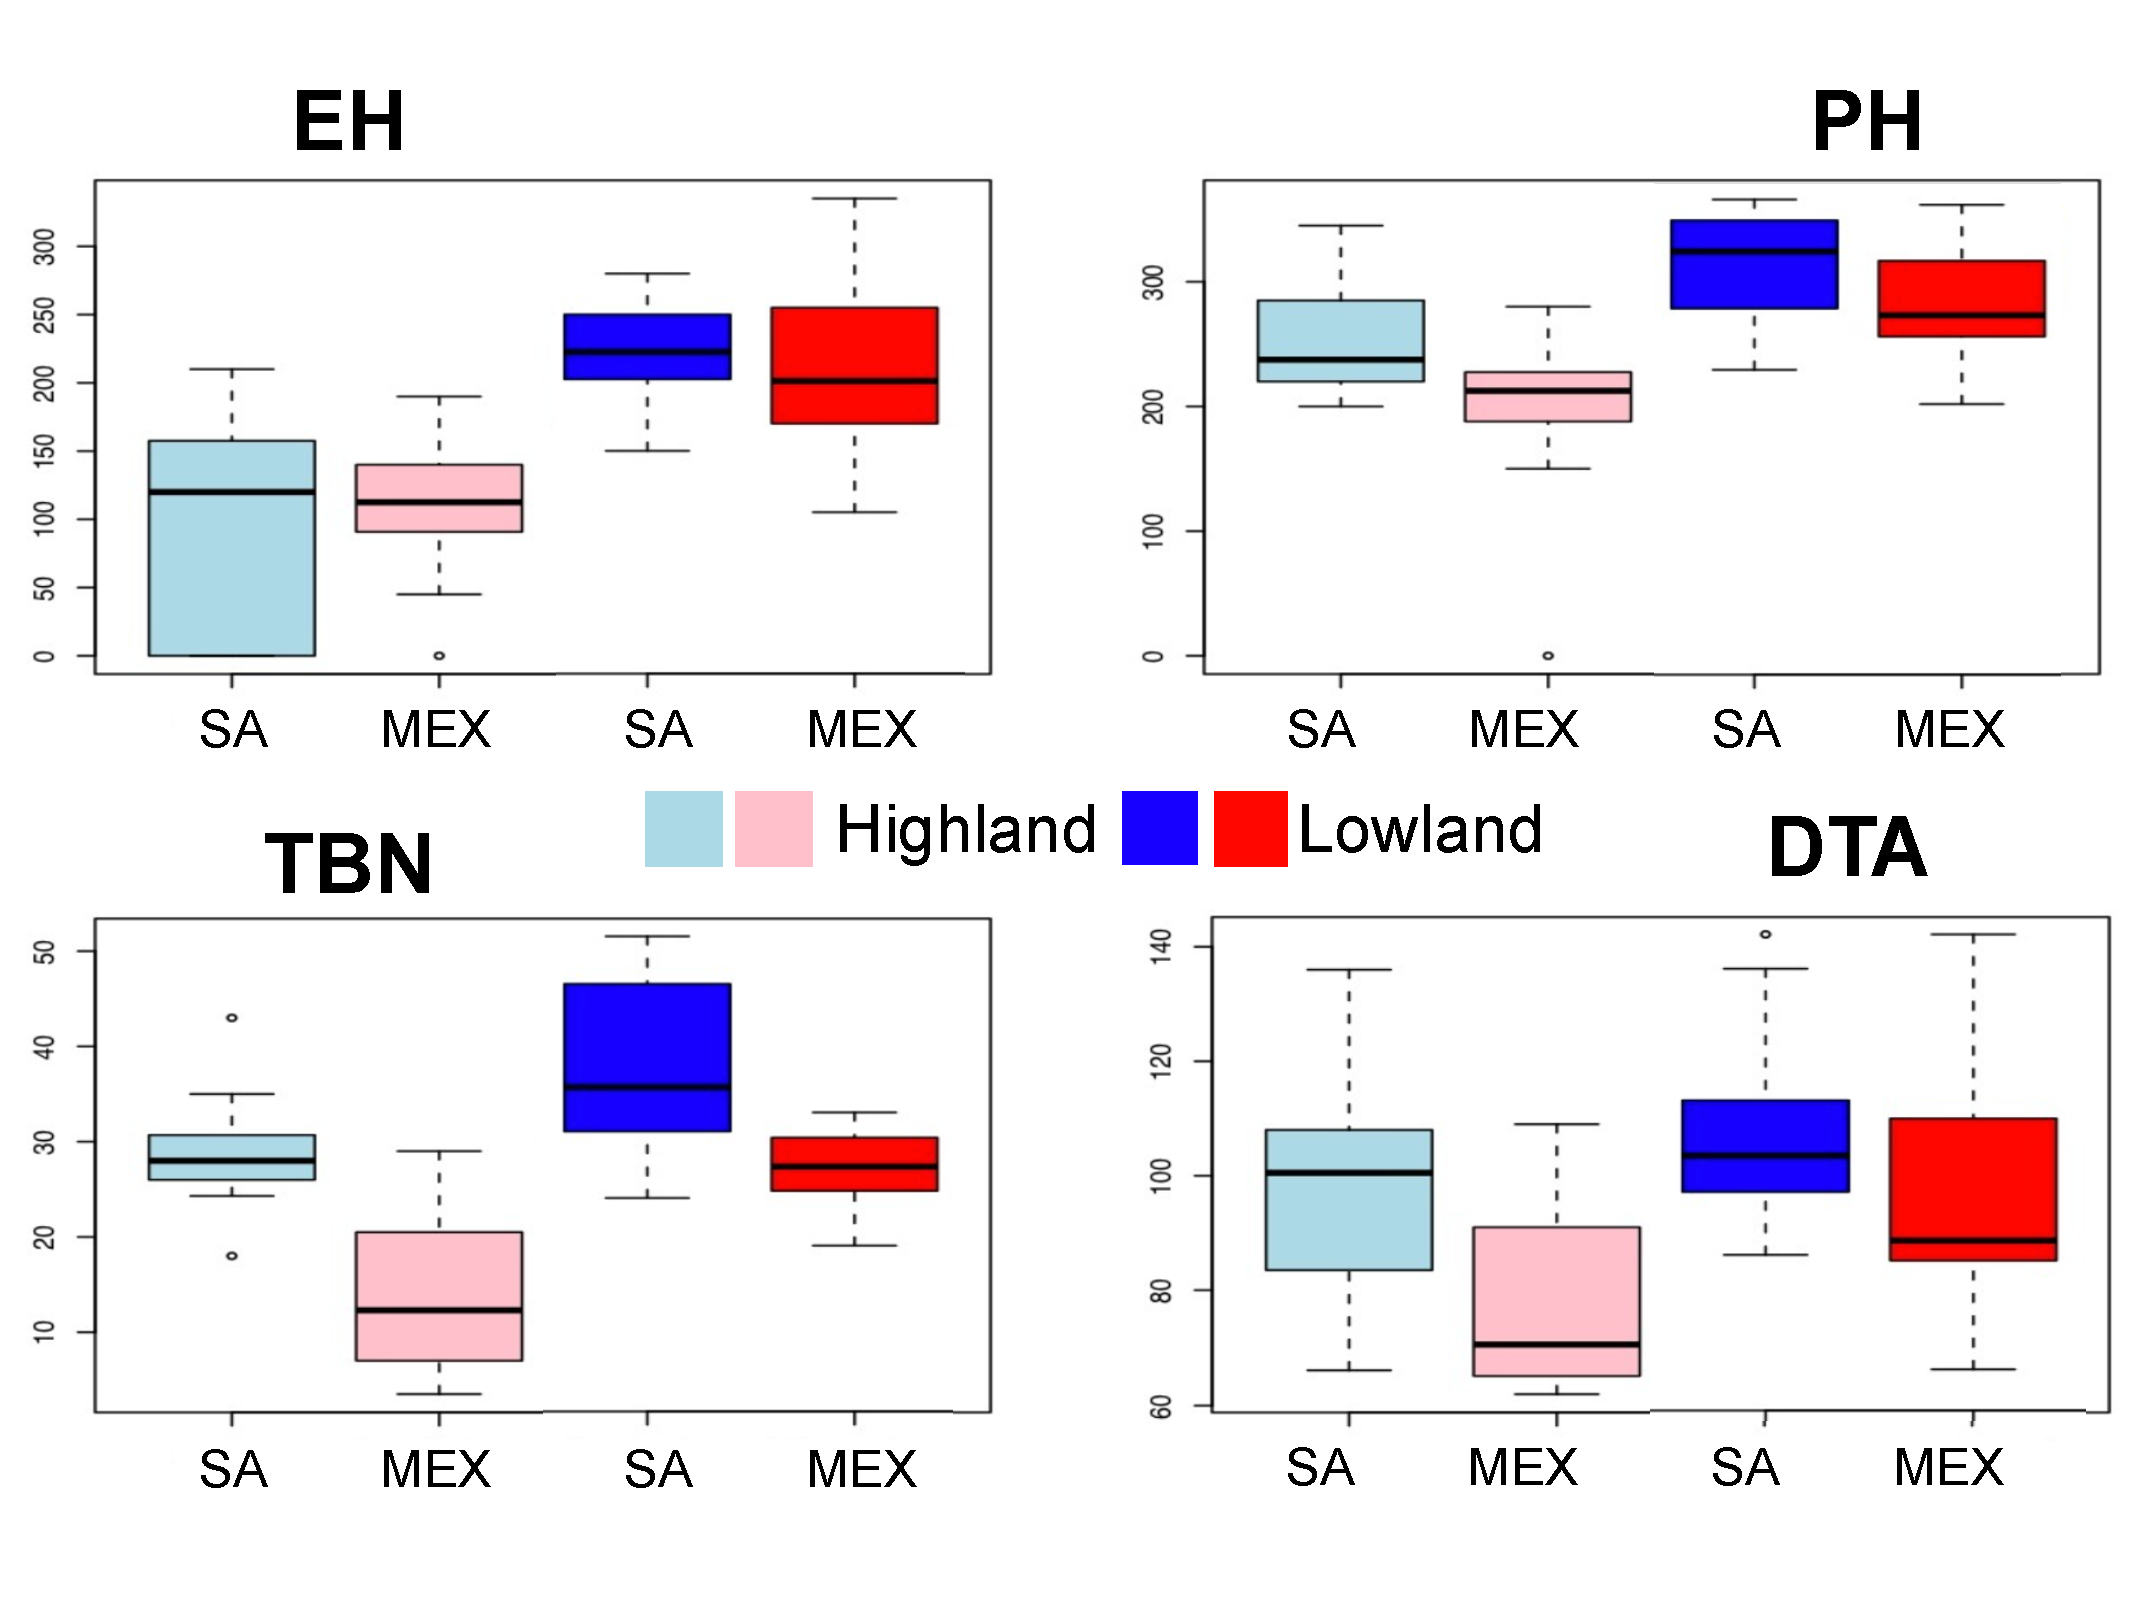
\includegraphics[width=0.5\textwidth]{fourtraits.pdf}
  \caption{Analysis of simulated admixed populations. 100 generations of admixture between \emph{mexicana} and \emph{parviglumis} were simulated for a 100cM chromosome.  The horizontal gray line represents the mean level of admixture along the chromosome.  A  beneficial \emph{mexicana} allele with selection strength $s=0.1$ was simulated at position 10cM (red vertical line), showing that variation in ancestry along a chromosome can be used to detect selection in admixed population. } 

\label{fig:fourtraits}
\end{figure}

\end{columns}
Raw data from each plot will be analyzed using mixed-models incorporating replications and environments.  Data will be analyzed across environments to determine whether location (elevation) affects the various phenotypes, as expected.  Each location will then be analyzed separately to derive least squares means to be used as the phenotypic data in QTL analyses.  QTL analysis will be conducted using standard, publicly available software (e.g. SAS; R/qtl \citealp{Broman2003a}).  Several iterations of QTL analysis will be conducted: on individual traits, individual traits adjusted for covariates such as flowering time, and multiple traits simultaneously.  The QTL profiles will be compared across populations (Mexican vs South American) and across field sites (elevations) to determine how elevation affects putatively adaptive traits.  We expect very different QTL profiles from the highland and lowland evaluation sites, and from the Mexican and South American populations.  Finally, the contrast of each Mexican location to the Missouri location will account for daylength differences and agronomic value in the Midwest. 

The expected outcomes of this objective will be 1) A map of QTL underlying phenotypic differences between highland and lowland maize in Mexico and South America, detailing the number and effect size of each QTL and differences between crosses, and 2) Estimates of fitness differences (PH, BM, SM, and FK \ref{tab:phenos}) of highland and lowland plants, as well as F2 with various combinations of QTL, in both environments. 

%Our expectations follow from the slow adaptation of each landrace to its specific environment (latitude, altitude, and other environmental factors). Finally, the contrast of each Mexican location to the Missouri location will account for daylength differences and agronomic value in the Midwest. One Genotypic studies of germplasm have repeatedly demonstrated that South American highland germplasm has been under-utilization in breeding programs (Goodman? ). The germplasm has been severely limited by inability to “move down the mountain,” which will likely parallel adaptation of other germplasm groups to changing environments.  

%this needs something else. needs to talk about how we will answer questions above. that we will find how many QTL for each trait, that we expect this wil vary from fitness (yield) to color, thus informing us about the lability of these traits and how selection (or breeders) may act on them. also needs to mention fitness, no?  can we not use these pops to tell which traits are adaptive (i.e. genetically correlated to fitness/yield?)

\subsection{Admixture mapping in a teosinte hybrid zone} \label{subsec:admixmap}
%\begin{itemize}
%\item collection trip (MBH)
%\item 500 individuals from Ahuacatitlan in Mexico (MBH, RS)
%\item DNA extractions, genotyping (MBH)
%\item phenotyping (MBH, RS)
%\item mapping (MBH/GC)
%\end{itemize}

% !HELP: writing



%%%%%%%%%%%%%%%%%%%%%%%%%%%%%%%%%%%%%%%%%%%%%%%%%%%%%%%%%%%%%%%%%%%%%%
%AIM 2
%%%%%%%%%%%%%%%%%%%%%%%%%%%%%%%%%%%%%%%%%%%%%%%%%%%%%%%%%%%%%%%%%%%%%%
\section{Adaptive value of highland alleles} \label{sec:selection}

In aim \ref{sec:qtl} we will map loci corresponding to traits differing between highland and lowland maize and teosinte. In this section we will investigate the evolutionary consequence of the QTL identified in \ref{sec:qtl} in three natural introgression experiments: gene flow from \emph{mexicana} into highland maize \ref{subsec:intropopgen} and admixture between \emph{mexicana} and \emph{parvgilumis} \ref{subsec:admixpopgen}. 

\subsection*{Questions}
\begin{itemize}[topsep=0pt,itemsep=-1ex,partopsep=1ex,parsep=1ex]
\item Are introgressed loci adaptive?
\item Does evidence of introgression and natural selection correspond to QTL?
\end{itemize}

\subsection{Global analysis of highland haplotypes} \label{subsec:global}

% !HELP: writing

%\begin{itemize}
%\item Occurrence of highland haplotypes/QTL/SNPs in global pops (MBH)
%\item 500 worldwide accessions GBS (MBH)
%\item Berg's approach to show selection on traits in multiple highland popualtions
%\end{itemize}

And though quantitative genetic theory suggests that adaptive phenotypic change may not correlate with strong evidence for selection on individual loci \citep{le2012genetic}, recently developed methods from Co-PI Coop \citep{Berg2013} provide a powerful statistical framework to identify coordinated shifts in allele frequencies at causative QTL (from \ref{sec:qtl} to look for weak selection on alleles underlying highly quantitative traits.  

\subsection{Population genetics of maize-teosinte introgression} \label{subsec:intropopgen}

Our previous work \citep{Hufford2013} we documented extensive introgression between \emph{mexicana} teosinte and highland maize landraces, demonstrating an overlap with teosinte QTL for macrohairs and stem pigmentation \citep{Lauter2004a}. Because of the relatively low-density genotyping used, however, we were limited to identifying large regions of ancient introgression present in most populations.  We were also unable to investigate evidence of selection for any of the introgressed regions.  Here we propose to revisit these populations with higher-density genotyping that will allow identification of ongoing gene flow in individual populations and ask whether introgressed regions have been targeted by natural selection.  

We propose to resample 18 individuals from each of the same 9 sympatric population pairs and two allopatric populations studied in \citet{Hufford2013}. Each individual will be genotyped by GBS \ref{Elshire 2011, Glaubitz2014} using greater than normal depth (48 plex) to improve genotyping heterozygous sites.  These data will provide \textasciitilde 1M SNPs across the genome (compared to 40K SNPs in \citet{Hufford2013}). We will use both haplotype \citep{price2009sensitive} and heterozygosity-based \citep{Geneva2014} methods to identify introgressed segments in individual populations.  Genomic regions showing evidence of introgression will be tested for selection using population genetic approaches which utilize evidence from the site frequency spectrum \citep{nielsen2005genomic} and haplotype structure \citep{voight2006map}.  Correlations between genetic differentiation and recombination will allow us to investigate selection against introgression \citep{Brandvain2013}, quantifying the "linkage drag" associated with introgression of potentially beneficial adaptive alleles.  Finally, we will again apply the approach of \citet{Berg2013} to evaluate selection on individual phenotypes across highland maize landrace populations.

The expected outcomes of this objective are 1) a fine-scale dissection of both ancient and ongoing introgression 2) identification of introgressed regions showing evidence of positive selection, identifying loci important for highland adaptation,  3) evidence for selection on specific phenotypic traits, 4) quantification of the potential "linkage drag" or evidence against introgression across otehr regions of the genome.

%GBS of 18 inds x 10 pops x 2 subspecies (mex \& maize) (JRI)
%384 at 48 plex * \$60 = \$23040

\subsection{Population genetics of hybridization in teosinte} \label{subsec:admixpopgen}

% !HELP: writing


\begin{SCfigure}
  \centering
  \caption{Analysis of simulated admixed populations. 100 generations of admixture between \emph{mexicana} and \emph{parviglumis} were simulated for a 100cM chromosome.  The horizontal gray line represents the mean level of admixture along the chromosome.  A  beneficial \emph{mexicana} allele with selection strength $s=0.1$ was simulated at position 10cM (red vertical line), showing that variation in ancestry along a chromosome can be used to detect selection in admixed population. } 
   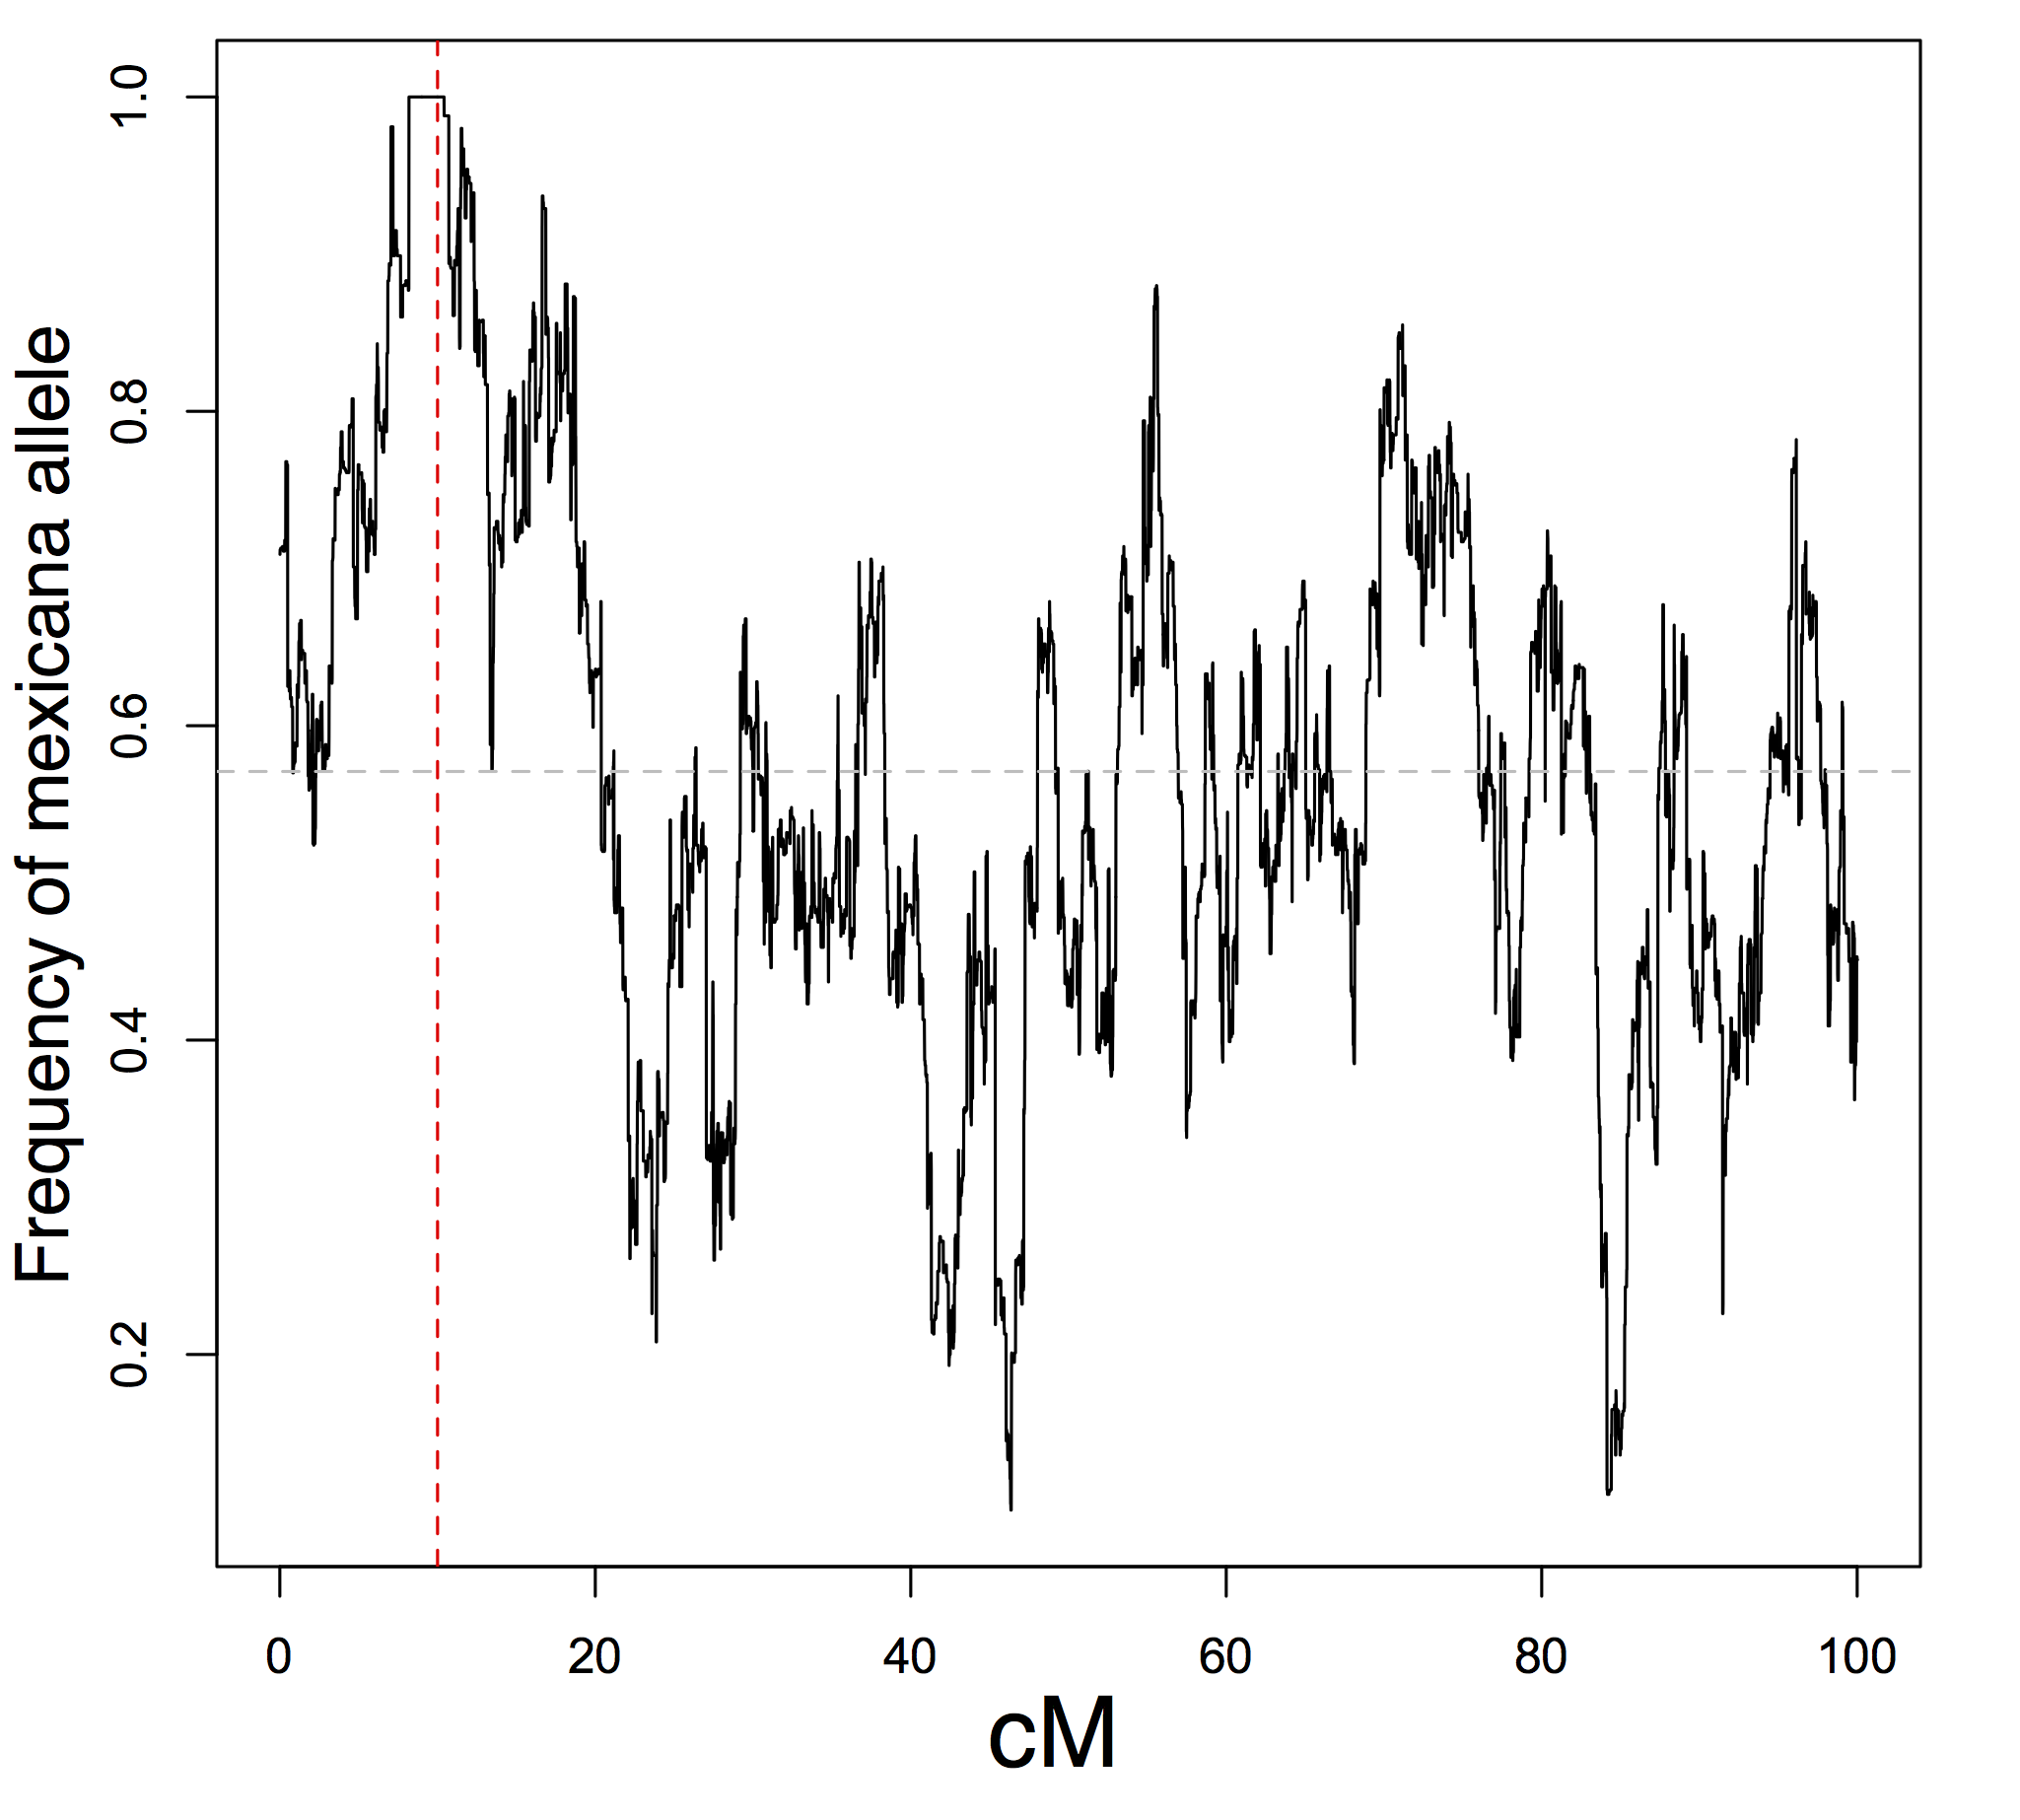
\includegraphics[width=0.5\textwidth]{admix.png}
\label{fig:cline}
\end{SCfigure}

make use of admixed pop sampled by matt
Berg approach of phenotypes mapped there for selection in parentals and hybrid

GBS Additional 5 admixed parv/mex populations (50 inds. each) (JRI)
also 4 new pops x (12 parv + 12 mex + 12 hybrids) = \$8160
Ahuacatitlan and 4 more
Introgression and adaptation in additional admix pops (JRI, GC)
Selection for/against regions in parv/mex/admix
Parallelism across pops in hybrid zone
yaniv figure here

%%%%%%%%%%%%%%%%%%%%%%%%%%%%%%%%%%%%%%%%%%%%%%%%%%%%%%%%%%%%%%%%%%%%%%
%AIM 3
%%%%%%%%%%%%%%%%%%%%%%%%%%%%%%%%%%%%%%%%%%%%%%%%%%%%%%%%%%%%%%%%%%%%%%
\section{Functional characterization of adaptive QTL} \label{sec:funchar}

After mapping QTL for highland adaptation (\ref{sec:qtl}) and studying their adaptive significance (\ref{sec:selection}), in this aim we will aim to better understand the functional genetic basis of adpative regions.  First, we will study the phenotypic effects of a chromosome 4 QTL introgressed into a maize background (\ref{subsec:nils}).  Then we will evaluate the effects of an allelic series from highland and lowland maize and teosinte at the chromosome 4 QTL (\ref{subsec:series}).  Finally, we will use RNA sequencing data to investigate plasticity, differences in expression, and identify potential candidate loci within QTL (\ref{subsec:rnaseq}).

\subsection{Questions}
\begin{itemize}[topsep=0pt,itemsep=-1ex,partopsep=1ex,parsep=1ex]
\item What are the phenotypic consequences of introgressing a single adaptive QTL?
\item Do adaptive QTL contain allelic series with differing functional consequences?
\item How do maize and teosinte data differ in expression response to higland and lowland environments?
\item Can RNA-seq help refine QTL to identify candidate genes?
\end{itemize}

\subsection{Functional evaluation of a Chr 4 QTL} \label{subsec:nils}

In this objective we propose to functionally characterize the genetics of a large \emph{mexicana}-maize introgression block located on chromosomes 4 (Chr4: 169-180Mb). Our previous analysis \citep{Hufford2013} indicates that this region is supported by a robust signature of introgression, shows broad distribution among highland races, and overlaps with a QTL identified in a \emph{parviglumis} x \emph{mexicana} cross  \citep{Lauter2004a} associated with leaf pigmentation and pubescence. Our previous population genetic analysis in teosinte \citep{Pyhajarvi2013}  suggests that the region represents an inversion polymorphism that is under selection along an altitudinal cline \ref{fig:cline}.  This suggesting the possibility of characterizing the region as a block by generation of introgression stocks.

\begin{figure}
  \centering
   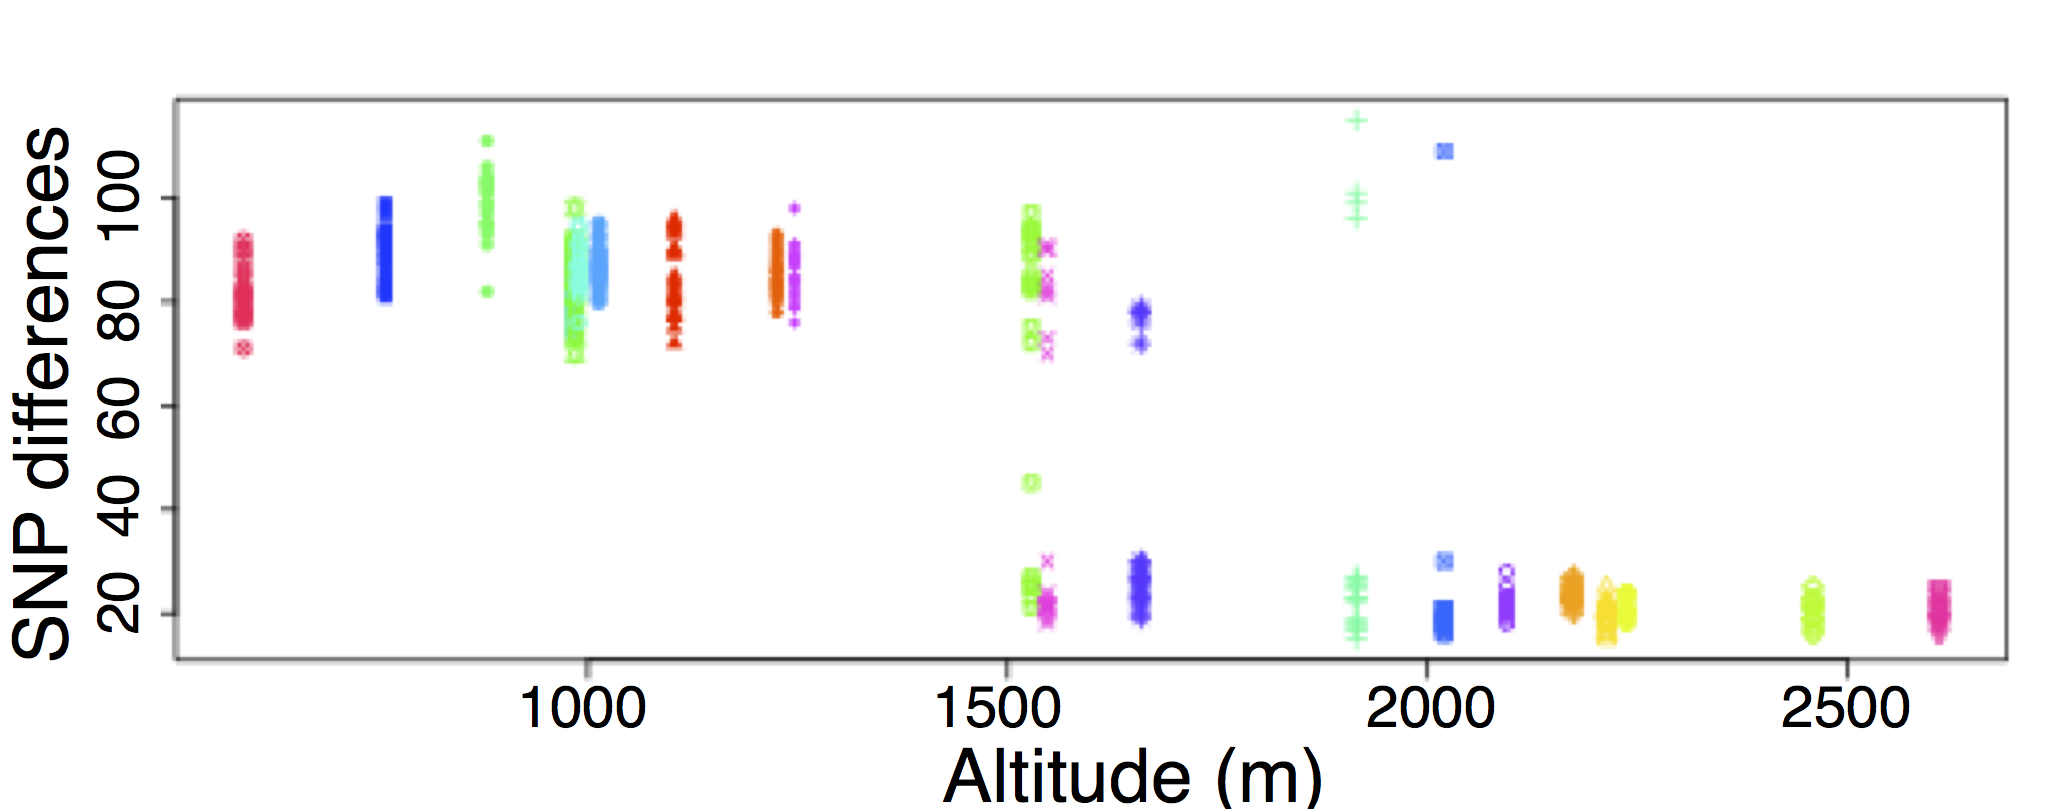
\includegraphics[width=0.7\textwidth]{chr4.png}  \caption{Clinal variation at the Chr4 inversion. Genetic distance (\# of SNPs) from the canonical highland haplotype is plotted against elevation for 20 teosinte populations (shown as different colors).  Low elevation (<1500m) populations lack the inversion completely, while it is fixed in populations abouve 2000m. Data from \citet{Pyhajarvi2013}. } 


\label{fig:cline}
\end{figure}

We will generate heterogeneous inbred families \citep[HIFS;][]{tuinstra1997heterogeneous} from a cross of the landrace Palomero Toluque\~no (PT) and the reference genome inbred B73.  PT is popcorn originating from the highland valleys of central Mexico that is considered basal to the Mexican highland landrace radiation \citep{reif2006grouping}; it also exhibits the highest level of \emph{mexicana} introgression among characterized material \citep{Matsuoka2002}. Furthermore, inspection of the PT genome sequence \citep{Vielle-Calzada2009} shows that PT carries \emph{mexicana} alleles at two SNPs shown previously to exhibit a fixed difference between  \emph{mexicana} and maize \citep{Hufford2013}. We will screen an existing collection of \textasciitilde 150 B73 x PT BC1S3 (three generations of selfing after 1 generation of back-cross) families to identify HIFs segregating for B73 and PT haplotypes using microsatellite makers we have shown distinguish B73 and PT alleles in this region. HIFs will be self-pollinated to generate pairs of near-isogenic lines (NILs) homozygous for the B73 or PT haplotype. While different in the candidate region, NIL pairs will share a common genetic background outside this region, including a sizable (~25\%) contribution of PT, capturing potential epistatic effects important to expression of the candidate phenotype. NILs will be genotyped by GBS  \citep{Elshire 2011, Glaubitz2014} both to confirm the extent of introgression at the Chr4 candidate locus and to characterize this shared background. A total of 6 HIF derived NIL pairs (i.e. 12 lines), will be characterized in our three field sites (Table \ref{tab:locales}) and evaluated for phenotypes described in (Table \ref{tab:phenos}). In each site, we will plant 3 replicate rows of our NILs and B73 and PT parents. Data will be analyzed broadly as described in \ref{sec:qtlmap}, both treating the introgression region as a single block, or considering individual markers.

The expected outcomes of this objective are 1) estimation of the contribution of differences at the Chr4 candidate locus to variation in a number of important phenotypes, 2) determination of the degree of phenotypic plasticity with respect to highland and lowland environments, 3) identification of differences in phenotypic effect among NIL pairs, indicative of background dependent epistatic interaction among genes.

\subsection{Allelic series for QTL of interest} \label{subsec:series}

To investigate further evaluate functional diversity in the Chr4 candidate region, we will generate a series of NILs by marker-assisted recurrent backcross to B73 using a collection of seven diverse donor varieties (parental lines of the mapping populations in \ref{subsec:qtlmap} shown in Table \ref{tab:qtlpops}; one each of inbred \emph{parviglumis} and \emph{mexicana}; and the highland landrace Palomero Toluque\~no). Each of these parents either have resequenced genomes \citep{Vielle-Calzada2009, Chia2012a} or will be sequenced as part of this project in  \ref{sec:qtl}.
% !HELP: writing and outcomes

Exotic donors have been selected on the basis of diverse origin, availability of genomic information and their use in other components of the project. To select for exotic haplotypes during introgression, we will use the SSR markers described above coupled with GBS. Our exotic donors include partially inbred and open-pollinated stocks. Where prior characterization has revealed multiple haplotypes to be present in a single stock, we will select the most common haplotype for introgression by analyzing multiple F1 plants and then selecting a single individual for the first backcross. BC4S2 families are projected to be available by the end of 2017 (Table X). 

\subsection{Gene expression} \label{subsec:rnaseq}

We will first assess the effects of high and low elevation environments on genome-wide expression differences to identify genes responsive to these environments.  We will grow the 8 inbred lines which serve as parents of our allelic series analysis in \ref{subsec:series} in a highland and lowland field site \ref{tab:locales}.  From each inbred we will sample leaf and root tissue from three plants at each of two time stages (seedling and flowering adult). Tissue will be flash frozen and sent to UC Davis for extraction and sequencing (multiplexed 12 individuals per lane of an Illumina HiSeq 2500) at the UC Davis Genome Center. Each individual will be barcoded, providing 3 biological replicates for each tissue/time/environment combination. We will assess differences in expression across environments and identify overlap between differentially expressed (DE) genes and QTL from \ref{sec:qtl}, loci showing selection identified in \ref{sec:selection}, and introgressed regions showing phenotypic differences in \ref{subsec:nils,subsec:series}.   These results will help narrow down potential candidate genes in QTL and serve as functional validation of loci showing population genetic evidence of selection in introgressed and admixed populations.  The data will also allow investigation of the relationship between phenotypic plasticity and adaptive change \citep[c.f.][]{Rosas26082013} via comparison of DE genes among environments for a single inbred to differences in DE genes among inbreds to ask whether genes showing a plastic response in unadapted material (lowland landraces, \emph{parviglumis} B73) show constitutive response in adapted lines (\emph{mexicana},highland landraces).  

Our second approach will be a targeted analysis of transcriptomic changes in the Chr4 NIL lines from \ref{subsec:series}.  Using NILs generated from each of the same 7 inbred donors (alongside an additional replicate of B73), we will evaluate shoot tissues of three plants sampled at seedling and flowering stage for each of the two genotypes (homozygous B73, homozygous donor).  Samples will be extracted and sequenced as described above. These analyses will allow us to refine potential candidate loci within introgressed segments of our NILs, moving us closer to a functional characterization of observed phenotypic differences. Whole-transcriptome comparison to the donor transcriptomes will allow us to differentiate between cis and trans regulation of expression within the Chr4 region, and analysis of co-expression networks \citep[c.f.][]{Swanson-Wagner02072012}, will highlight the effects of introgressed genes on expression patterns in the rest of the genome, enabling us to begin to dissect the genetic pathways involved in adaptive highland traits.

The expected outcomes of this objective will be 1) Identification of candidate genes showing plastic differential expression within lines across environments 2) Identification of candidate genes showing differential expression among lines from different environments 3) Detailed information on the effects of introgressed segments on genome-wide expression. 

%\begin{itemize}
%\item Time series analysis of plants in field (ACJ):
%\item 15 Lines
%\begin{itemize}
%\item 4 F2:3 parents
%\item 1 NIL chr4,
%\item 1 each mex \& parv TIL
%\item B73, CML457, T43, PT
%\item highland/lowland landraces used in allelic series (MBH to inbreed)
%\end{itemize}
%\item 12 plants per line per environment (2 pools of 6)
%\item 4 stages/tissues per plant
%\item 2 environments (high/low fields)
%\end{itemize}

%To identify genes in maize that respond to highland environments conditions, we propose a transcriptome-based integrated approach based on field and greenhouse experiments. We will intersect phenotypes within a genotype with those across a panel of genotypes to uncover genetic variation underlying phenotypic plasticity associated to highland adaptation. We tested this approach sucessfully in Arabidopsis and found that genes that enable a functional response to the environment via phenotypic plasticity within a genotype underlie adaptive changes across genotypes (Rosas et al 2013). We will first generate transcriptomes from the reference genotype B73, a recurrent parent in the development of NILs (Aim 3.1). We will grow 90 plants in each of several sites that represent the environmental gradient of low to highland maize in Mexico. Three lowland sites (Valle de Banderas, Irrigated Winter; San Juan de Abajo, Irrigated Winter; Ameca, Rain Summer; two mid-elevation (Irapuato, Irrigated Summer, Celaya; Rain Summer and three highland sites (Amealco, Toluca, Texcoco all Rain Highland). Phenotypic data will be gathered as in Aim 1.1. We will plant one set of 30 plants at the beginning of the month during three months in 2015 (90 plants/genotype/environment) to obtain replicates that represent variability in these local environments. From each set we will sample leaf and root tissue at the 8-leaf stage from four plants for a total of 192 samples (2 tissues x 4 plants x 3 dates x 8 sites). Each of the sites will be characterized environmentally locally and with information from INEGI (Mexico) and from raster-formatted climate data from the Worldclim database. This experiment represents our ‘Field Environment’. 

%Our hypothesis is that significant gene expression changes observed in the B73 reference genotype will suggest plastic mechanisms that better adapt the plant to lowland and highland enviroments. Furthermore, we predict that in genotypes adapted to either the lowland or highland niche, many of these transcriptional changes will be constitutive with respect to the B73 reference. To test this, we will generate transcriptomes from locally-adapted genotypes growning in one controlled environment. We will grow genotypes that represent an array of phenotypic and genetic variation in maize, including key targets in this proposal: B73; Palomero Toluqueño; four parents of our F2:3 mapping population (Aim 1.1); CML457, T43 (Aim X); B73 NILs Chr 4 (Aim X); the highland/lowland landraces used in the allelic series (Aim 3.1); and mexicana and parviglumis teosintes, as well as three individuals from their admixed populations (Aim 2.1) for a total of 16 genotypes. Phenotypic data will be gathered as in Aim 1.1. We will generate transcriptomes from six biological replicates from shoots and roots from each genotype at the 8-leaf stage, for a total of 192 samples. This experiment represents our ‘Greenhouse Environment’
%We will identify the subset of climate variables that best summarizes each environment in our Field Experiment using a principal components (PC) analysis \citep{Yoder17012014}. Variance in expression patterns, topologies of coexpression networks and other analyses will identify genes whose expression and co-regulation is altered in the three environmental conditions (Swanson-Wagner et al 2012). Candidate genes underlying variation in Highland Adaptation will be those genes that behave as outliers from standing variation in the maize pan-transcriptome \citep{Hirsch01012014, Swanson-Wagner02072012} and in this set of experiments, and that are common only in and in all Highland sites. Genes overrepresented in candidate adaptive regions (e.g. Chr4; QTL identified in Aim X) are especially interesting. 
%A key premise here is that accessibility of the phenotypic plasticity space of a single genotype (B73) depends on the activity of the same genes controlling variation across many other genotypes within a species citep{Rosas26082013}. To test this principal components of the phenotypic data from the ‘Field Environment’ and the ‘Greenhouse Environment’ will be correlated using a mixed model to the a) main environmental variables from the Field Experiment; b) to GBS (Aim 2) and c) transcriptome-based SNPs (Swanson-Wagner et al 2012 & this study) to identify genetic variants that explain the variation in Highland conditions \citep{Rosas26082013}. By projecting one experiment onto the plasticity space of the other, it will be possible to identify gene expressin patterns that are shared among and within genotypes.
%Downstream tests can evaluate if mutants in candidate genes involved in phenotypic plasticity exhibit atypical phenotypic responses to their respective environment, exploring the functional mechanism of these genes citep{Rosas26082013}. Candidate genes can be re-sequenced in field populations and Highland landraces of various environments throughout Mexico and analyzed with a landscape genetic framework. Finally, transcriptomes generated here in addition to recently published transcriptome data for maize can enable a phylogenomic approach to identify the origin and functional importance of Highland Architecture genes in other plants \citep{lee2011}. 










\rowcolors{2}{gray!25}{white}
\begin{table}[H]
\begin{center}
\caption{Proposed timeline of activities and responsibilities}\label{tab:timeline}
\begin{tabular}{lccccc}\\\toprule  
    \rowcolor{gray!50}
Year & 2015 & 2016 & 2017 & 2018 & 2019 \\\midrule
Objective \ref{subsec:series} Allelic series & 2015 & 2016 & 2017 & 2018 & 2019\\\midrule
Objective \ref{subsec:nils} Fine mapping & -- & RS, AC & AC,JRI & AC,JRI & -- \\\midrule
Objective \ref{subsec:rnaseq} RNA-seq & 2015 & 2016 & 2017 & 2018 & 2019\\\midrule
Objective \ref{subsec:intropopgen} Maize/mexicana introgression & 2015 & 2016 & 2017 & 2018 & 2019 \\\midrule
Objective \ref{subsec:admixmap} Admix mapping & 2015 & 2016 & 2017 & 2018 & 2019 \\\midrule
Objective \ref{subsec:qtlmap} QTL mapping & 2015 & 2016 & 2017 & 2018 & 2019 \\\midrule
Objective \ref{subsec:global} Highland haplotypes & 2015 & 2016 & 2017 & 2018 & 2019 \\\midrule
Objective \ref{subsec:admixpopgen} Admixture population genetics & 2015 & 2016 & 2017 & 2018 & 2019\\ \bottomrule
\end{tabular}
\end{center}
\end{table} 


\required{Broader Impacts}
% As in the project summary, broader impacts must be called out separately 
% in the project description.  You may be able to give more specific
% examples, or discuss how you've previously achieved these impacts.
% It should be similar, but not identical, to the Broader Impacts statement
% in the project summary

%Also mention online presence?  twitter, online dissemination, etc.? slideshare, figshare, preprints, Haldane's sieve?

\subsection*{Exchange Program} 

We propose an international student exchange program between the PIs in the U.S. and Senior Personnel at LANGEBIO in Mexico. Over the course of the grant, we propose to fund 10 graduate or undergraduate students for 3-month research internships in one of the collaborating laboratories. Students involved will participate in research projects directly relating to the research focus of the grant, including developing mapping populations, mapping traits, population genetic analysis, or analysis of next-generation data. The expectation is that such research will often lead to co-authorship on publications. Students will be asked to give two presentations, one to the host lab upon arrival, talking about the lab/university they came from and research there, and another to their host lab detailing their work over the 3-month period.  Each of the PIs will participate, sending students to Mexico and/or accepting students from Mexico for internships. PI Ross-Ibarra will manage the program, as he is fluent in Spanish and has past experience with a similar exchange program (NSF 0922703). Over the last four years, his lab has hosted 6 Mexican students who have worked on various computational aspects of centromere evolution. Two of those students have earned authorship on a paper to be submitted later this year and one has gone on to a PhD program in the U.S.

Our goal is to involve students directly in research while at the same time fostering intercultural exchange and promoting future international research opportunities. It is particularly appropriate for the study of maize, a crop with significant cultural and economic impact in both Mexico and the U.S. Participating Mexican students will learn new analytical methods -- especially computational management of large datasets -- that can be introduced to their respective laboratories and peers. American exchange students will similarly benefit from experience with large field experiments and efforts to functionally characterize individual loci.  The hope is that Mexican undergraduate students involved may be recruited to graduate programs in the U.S., ideally to work in the lab of one of the PIs, and that American undergraduate students will be exposed to international opportunities for research, graduate education, and collaboration.

\subsection*{Phenotyping workshop} %SFG, JRI

The USDA-ARS group in Columbia has developed a streamlined phenotypic data collection system utilizing a handheld barcode device, barcoded plant tags, and barcoded phenotyping tools in order to maximize efficiency.  We will host a phenotyping workshop in Columbia during each year of the grant.  Through this workshop, Dr. Flint-Garcia’s state-of-the-art system will be transferred to other research institutions to aid in large-scale data collection. The phenotyping workshop will include topics on Experimental Design, setting up the FieldBook database, and Data Collection.  Experimental design topics include understanding where variation comes from, how to control for environmental/field variability and experimental error; heritability and repeatability.  The need for consistent data collection and high-throughput will be emphasized.  FieldBook database setup topics include setting up Palm handheld users, locations, traits, projects, assigning plots to projects, assigning traits and measurements to projects,  generating barcoded plant tags, and loading the program and trait groups to the Palm to prepare for data collection.  Topics to be covered in Data Collection include data collection for specific traits related to local adaptation of interest to our group, synchronizing data from the palm with the desktop/laptop database, managing data conflicts between the palm and the database, running reports, and exporting data.  This proposal will provide travel support for instructors.  The workshop will be free but participants will be expected to purchase their own Palm handheld and pay for their own travel.  The workshop will be held each year in late summer so that the participants can gain hands-on experience in data collection in the corn field.

\subsection*{Software} %JRI and GC

A good understanding of population and quantitative genetics is key to a student’s understanding of genetics and evolution, but these subjects are often conceptually quite difficult. An understanding of genetic variation and its phenotypic effects is also an increasingly important part of being an informed citizen, due to the rise of personal genomics and genomic medicine \citep[e.g.][]{redfield2012}. The large amount of population genetic and association data being generated offers a superb chance to motivate these subjects using real data. 
We will develop undergraduate teaching modules in population and quantitative genetics using data from this project. These modules will be tested and integrated into large undergraduate teaching courses (introductory evolutionary biology and genetics) at UC Davis and graduate courses at UC Davis and Iowa State (ecological genomics). We have already begun to develop and distribute some of these resources, e.g. genome-scale demonstrations of Hardy Weinberg Equilibrium (HWE) using  human HapMap data. Such demonstrations underscore the usefulness of basic population genetics in describing real world patterns, and begin to expose students to the wealth of genomics data being collected. 
Other examples will include: using association data from our admixed populations to demonstrate quantitative genetics models; and explaining concepts of genetic and genealogical ancestry using genomic identity by descent.  These modules will be prepared in the open source statistical program R, to ensure that they are easily used, modified, and distributed, and to expose students to programming in biology. The modules will be designed so that they can be tailored for use at a variety of levels from teaching basic concepts to large undergraduate classes to providing the raw data for programming exercises for upper division courses.

The modules will be publicly distributed via Github (see Data Management Plan) in a fully open manner. The use of github will allow others to modify and extend the modules and to share and track these modifications. 

\subsection*{Germplasm resources} %MBH, SFG and RS
%The highland environment remains an important niche for global maize production, in terms of acreage and farmer involvement, if not overall yield. The highland environment presents a number of important abiotic challenges beyond high elevation per se, including periods of drought and cold, and highland adapted material has great potential to provide an important source of stress tolerance; the rapid development and inherent earliness of highland material, for example, may have general application in marginal environments. 

This project will generate multiple germplasm resources.  Seed from the F2 parents will allow additional use of this mapping population to study additional phenotypes of interest (e.g. root morphology and growth).  Seed from our NIL populations will allowing investigation of genome-wide introgressions from a variety of exotic lines.  Such material could be of interest to the Germplasm Enhancement of Maize (http://www.public.iastate.edu/~usda-gem/) project as well as to public and private breeders both in the US and abroad. In Mexico, for example, the highland niche represents a key target market for an emerging private sector of small breeding companies established following deregulation in 1990s. While highland adapted hybrids are available, these are largely derived from lowland sub-tropical material with little or no contribution of the highland landraces and the germplasm developed here could be an important contribution to furthering such programs. Finally, seed from our collections of teosinte will enhance the sampling of these subspecies and provide additional diversity not currently present in germplasm banks.  Seed from our mapping populations will be deposited in the USDA-ARS Maize Stock Center at the University of Illinois, and backups will be kept at Iowa State and Missouri.

%This project will also build further the collaboration between US institutions and LANGEBIO, with a number of Mexican graduate students being directly involved. While Mexican plant science retains a traditionally strength in biochemistry and molecular biology, genetics has been less well represented in recent years. As a consequence, while there is ready access to genomics technologies, the human resources to make the most of the opportunities they present may be lacking. This project provides an excellent opportunity for capacity building in a Mexican institution, with the expectation of a lasting impact through future collaboration.

\required{Results From Prior NSF Support}
% 5 pages or fewer of the 15 pages for entire description document.
% include results from NSF grants received in the past 5 years.
% If supported by more than one grant, choose the most relevant one.

% For each grant, include: 
%	(a) NSF award number, amount, dates of support 
%	(b) The title of this project
%	(c) Publications resulting from this research
%	(d) Summary of the results of the completed work
%	(e) A brief description of data samples available and other research products not described 	      elsewhere
%	(f) For renewed support, a description of the relationship between the completed and 			      proposed work

% Due to space limitations, it is often advisable to use citations rather
% than putting the titles of the publications in the body 
% of this section

\subsection*{Ross-Ibarra, Flint-Garcia: \#1238014: Biology of Rare Alleles in Maize and Its Wild Relatives}
\$13,311,185 (\$2,368,767 to Ross-Ibarra and \$1,206,211 to Flint-Garcia), 05/15/13-04/30/18. PI Edward Buckler, co-PIs J. Doebley, J. Holland, S. Flint-Garcia, Q. Sun, P. Bradbury, S. Mitchell, J. Ross-Ibarra
\par\noindent{\bf Intellectual merit} In the first year we have developed accurate imputation approaches, found evidence for the importance of deleterious variants and non-genic polymorphisms in heterosis and GWAS, documented differences in recombination among the parents of the NAM population, and found population genetic evidence suggesting the importance of demography and purifying selection across the genome.  The grant has produced 18 total publications in its first year (only publications involving PIs Flint-Garcia and Ross-Ibarra are shown below). 
\par\noindent{\bf Broader impacts}  In the first year this project has included 10 postdoctoral and 12 graduate trainees. The GBS workshop and traveling maize exhibit continue to be popular and successful. A new version of the teacher-friendly guide to the evolution of maize has been revised and published online. 
\par\noindent{\bf Publications} \citet{peiffer2013genetic, Romay2013, wills2013many, Mezmouk2014, Peiffer2014, sood2014mining}

\subsection*{Ross-Ibarra: \#0922703: Functional Genomics of Maize Centromeres}
\$5,008,031 (\$754,409 to Ross-Ibarra). 09/01/09-08/31/14. PI Kelly Dawe, co-PIs J. Birchler, J. Jiang, G. Presting, J. Birchler, J. Ross-Ibarra
\par\noindent{\bf Intellectual merit} Centromeres are regions of the genome that organize and regulate chromosome movement, yet the biology of centromeres remains poorly understood. Co-PI Ross-Ibarra's group has focused in particular on the evolutionary genetics of centromeres. This work has demonstrated the remarkable evolutionary lability of centromere tandem repeats, but has shown that there is little evidence in maize for coevolution between centromere sequence and kinetochore proteins. Ongoing work from the Ross-Ibarra lab seeks to characterize kinetochore proteins, assess the phylogenetic evidence for longer-term coevolution, and understand patterns of centromere and genome size variation in natural populations.
\par\noindent{\bf Broader impacts}  Co-PI Ross-Ibarra has established and currently runs an international student exchange program as part of this grant. Data and result of this project have been disseminated via publications and presentations as well as deposited in the maize genetics community database \url{www.maizegdb.org}. Former trainees on the grant include Dr. Matthew Hufford (Co-PI on the current grant). 
\par\noindent{\bf Publications} \citet{Shi2010a, Chia2012a, Fang2012a, Hufford2012, Hufford2012b, Hufford2013, Melters2013a, Kanizay2013, Pyhajarvi2013}

\subsection*{Coop: \#1262645: Collaborative Research: ABI Innovation: Visualization And Statistics For Spatial Population Genomic Analysis. }
\$314,260, with an effective date of 05/01/13. Award Duration: 36 months.
\par\noindent{\bf Intellectual merit} We are developing a set of spatial statistics methods based on Gaussian random fields for the analysis of geographic population genomics data. The first method based on this approach has just been published, allowing a sound statistical framework to distinguish the effects of geographic and ecological distance on genetic isolation. 
\par\noindent{\bf Broader impacts}  The R package of the software has been released online, and has already been used by many molecular ecologists. 
\par\noindent{\bf Publications} \citet{bradburd2013}

\subsection*{Flint-Garcia: \#0820619: Genetic Architecture of Maize and Teosinte}
\$ 9,823,000. 3/1/2009-2/28/2013. PI Edward Buckler, co-PIs J. Doebley, T. Fulton, S. Flint-Garcia, J. Holland, S. Kresovich, M. McMullen, Qi Sun. 
\par\noindent{\bf Intellectual merit}  This project extends over more than a decade, and has pioneered the characterization of population genetic and evolutionary parameters of maize diversity, developed resources to connect this genetic diversity to phenotype through both association and joint linkage-association mapping, conducted fine scale analysis of domestication and agronomic QTL, and recently expanded to whole-genome analysis of diversity, evolution, and phenotype. Overall, the maize diversity project has developed a wide range of approaches and broadened understanding of the maize genome, evolution and adaptation, genetic mapping, and the agricultural improvement of maize. The project successfully released and analyzed the maize Nested Association Mapping (NAM) population, collaborated on making first and second generation haplotype maps for maize, resolved domestication traits, developed a range of novel statistical approaches for association mapping, and dissected complex traits such as flowering time, kernel composition, disease resistance, height, and inflorescence and leaf morphology. 
\par\noindent{\bf Broader impacts} The outreach program included a traveling science museum exhibit on maize diversity, evolution and genetics (seen by at least 300,000 people at five venues to date, including the famous Corn Palace in South Dakota), online Teacher Friendly Guide to the Evolution of Maize, seven Genotyping-By-Sequencing (GBS) workshops (held at primarily at Cornell but has also been held in Kenya), and training of postdocs, graduate students and undergraduates, the vast majority of which have continued in scientific careers.  Former trainees on this grant include Dr. Flint-Garcia  and Dr. Ross-Ibarra  (PIs of the current grant), only their publications are shown below.
\par\noindent{\bf Publications} \citet{Buckler2009, Flint-Garcia2009, Flint-Garcia2009a, Flint-Garcia2009b, Gore2009, McMullen2009, Ross-Ibarra2009a, Bottoms2010, Dubois2010, Zhang2010a, vanheerwaarden2010a, vanheerwaarden2010b, Brown2011b, Morrell2011a, Studer2011b, vanheerwaarden2011a, Tian2011, Chia2012a, Cook2012a, Fang2012a, Hufford2012b, Hung2012, Hung2012a, Romay2013}
